\documentclass[11pt]{article}
\usepackage[utf8]{inputenc}
\usepackage[T1]{fontenc}
\usepackage{graphicx}
\usepackage{longtable}
\usepackage{float}
\usepackage{wrapfig}
\usepackage{soul}
\usepackage{amssymb}
% \usepackage{hyperref}


\title{Architectural Design Document\\
  Software Engineering Project Course\\
  Naamakahvi\\
  University of Helsinki}

\author{Antti Hietasaari
  \and Joonas Magnússon
  \and Irina Mäkipaja
  \and Samir Puuska
  \and Janne Ronkonen
  \and Eeva Terkki
  \and Ossi Väre}
\date{\today}

\begin{document}

\maketitle

% \setcounter{tocdepth}{3}
\tableofcontents
% \vspace*{1cm}



\section{Introduction}
% \begin{itemize}
% \item High-level description of overall architecture
% \item Main functionalities described in natural language
% \end{itemize}

The staff of the Department of Computer Science has two coffee syndicates. 
Both of them provide an espresso machine and the other syndicate also has 
a drip coffee maker. The members pay for their coffee by bringing products 
to be used in the machine, e.g. espresso beans or filters. The Facecafe 
software keeps track of each member’s balance, using face recognition to 
identify users. The software can be used on an Android tablet
or a desktop computer and it is supposed to replace other methods for track 
keeping. Facecafe uses the old database of Coffee Touch software, a system 
that has earlier been used for the same purpose.

Registration is required to use the system. Upon registration, pictures are
taken of the user's face for later identification. If the user does not want
to use face recognition, they can choose not to have any pictures taken. 
Images can also be added after registration. Coffee can be bought or paid for 
by first choosing a product to buy or bring and then taking a picture to identify
the user whose balance will be updated. Alternatively, the user can be identified 
using their username. 

In this document, coffee syndicates that are connected to the same server are 
referred to as stations.
\section{System Purpose: Requirements}

\subsection{Functional Requirements}
   % --> Bullet point list
   % --> e.g. must be able to bill customer credit cards, must be able to
   % insert a code snippet to customers site. etc.

\begin{itemize}
\item{The user can register on the system}
\item{The user can be authenticated using face recognition}
\item{The user can be authenticated using their username}  
\item{The user can buy one or more coffees}
\item{The user can bring products}
\item{The user can check their balance}
\item{The user can add new images after registration}
\end{itemize}  

\subsection{Non-functional Requirements}
   % --> Bullet point list
   % --> e.g. expected unit test ratio, expected test coverage, expected
   % performance

\begin{itemize}
\item{The application can be used on an Android tablet or a desktop equipped with a touch screen}
\item{The software is simple to use and the core functionalities do not require many clicks}
\item{The software works reasonably fast} 
\item{Simplicity of use is more important than security (the coffee syndicate is based on trust)}
\end{itemize}

\section{Structure}

\subsection{Overview: Overall Structure}
% --> Diagram of all components and their collaboration with each other
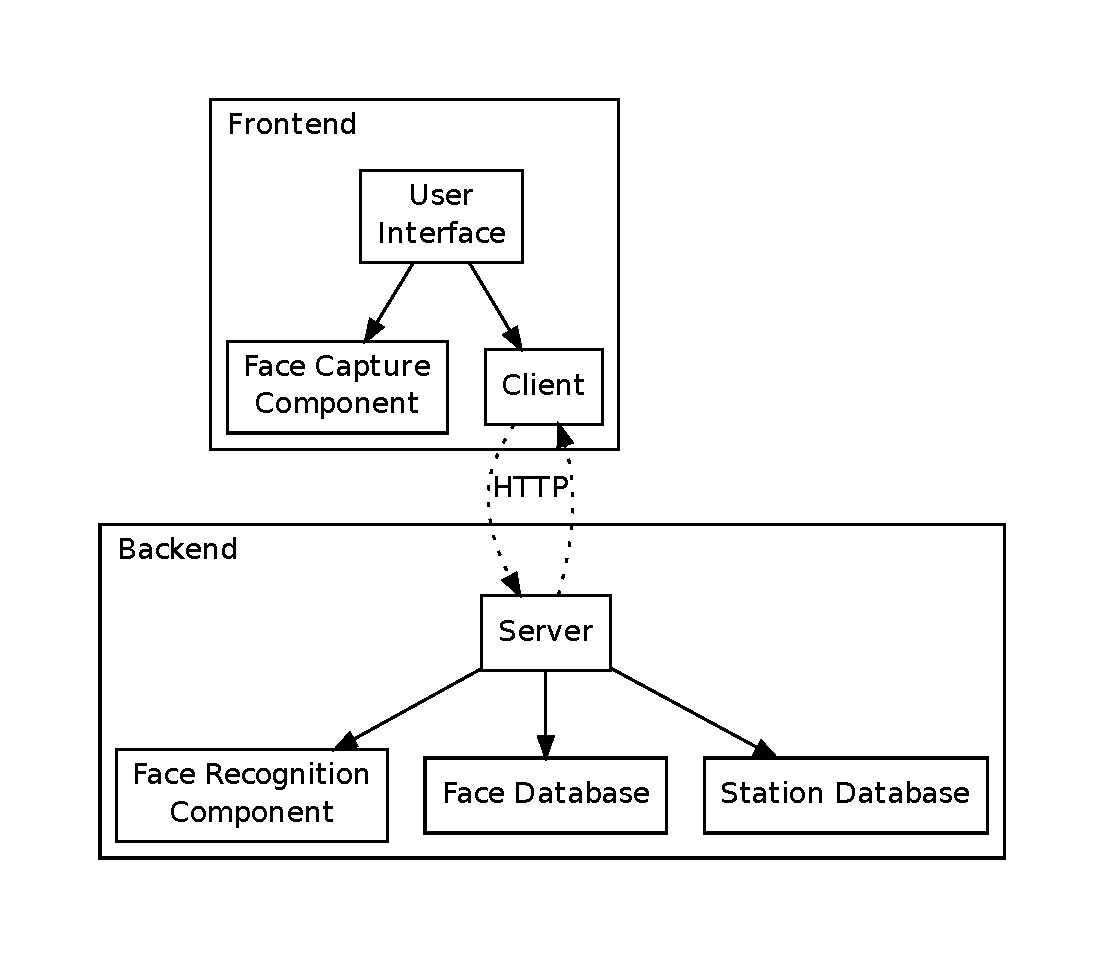
\includegraphics[scale=0.5]{components.pdf}\\
The software is divided into a frontend and a backend. The frontend consists of a user interface,
a face capturing component (which is a part of the user interface) and a client. The backend has
a server, a component for face recognition and two kinds of databases, one for images of the users'
faces and the other for information related to a specific station.

\subsection{Components}
   % for each component:
   %   - description of the component
   %   - components responsibilities
   %   -interfaces that the component offers
   %   - constraints
   %   - collaboratoring components
   %                for each collaborating component:
   %                  -  description of the collaboration
   %                  - interfaces used
   %                  - constraints

   % --> Just short listing of every component what should say,
   % e.g.
   % KujeProcessor is responsible for XX and YY, 
   % interfaces: removes processed data from kuje-table, inserts data for WebApp,
   % collaborates: with KujeServer and WebApp, but KujeServer does not
   % collaborate (directly) with WebApp.
   % collaborates:
   % KujeServer: takes kuje records from KujeServer database and afterwards
   % removes them
   % WebApp: updates the reports which are represented by WebApp
   % for each component interface:
   %   - description of the interface
   %   -  operations
   %   - constraints on the order of operation


\subsubsection*{Swing User Interface}
% swing-ui ihmiset voisivat kirjoittaa tästä enemmän (myös frontendin opencv-juduista)
     
The Swing user interface is written in Java and provides an interface
between the users and the server. The UI shows product and user account
information stored on the server and allows users to manage account
and purchase information.

The Swing user interface is designed to operate on Windows, Linux and
Mac devices. It does not communicate with the backend directly, but rather
uses the client library to facilitate communications with the server.
It also uses the third-party OpenCV and JavaCV libraries to detect faces
from a camera feed. The faces are sent to the server in order to identify
users, allowing them to sign in to the system without entering their
usernames or other information.

\subsubsection*{Android User Interface}
% android-ui ihmiset voisivat kirjoittaa tästä enemmän (myös frontendin opencv-juduista)

The user interface for Android is written in Java, and uses the client
library to facilitate communications with the server. It also uses the OpenCV library for face detection.

The Android user interface was designed for a 10.1" screen in landscape mode, but should be transferrable to other types of screens with little effort. A physical (Bluetooth) keyboard is recommended for inputting user details, although the Android virtual keyboard can also be used.

\subsubsection*{Client/Frontend}
The client is implemented as a Java library and its responsibility is
to offer an interface for UI-components, abstracting away the
communication protocols used between the client and server. The client 
communicates with the server via HTTP, sending GET and POST requests, 
and receiving JSON-objects from the server. 

For a more detailed description, see the client Javadoc.

\subsubsection*{Backend/Server}
% redox ja mahnu vois varmaan kirjoittaa tähän jotain tarkempaa, ja
% ehkä jakaa tämän kohdan useampaan kohtaan jos siltä tuntuu. (+ naama- ja station-tietokannat ja serverin opencv-palikka)
The server consists of a server module, several databases along with their own database modules and a module for open-cv. 
The server module uses the database modules, that update and read the databases, and communicates with clients via HTTP.
Databases are PostgreSQL and their modules use the psycopg library. SQL statements are stored in an XML document and are
parsed by the database modules. There is one database for every coffee station, because
products and balances vary. Facial recognition is done by the open-cv module. 

\section{Dynamic Behavior}
\subsection{Scenarios}
% for each scenario:
% - type: system operation or use case
% - description of the scenario
% - how scenario interacts with components

% kuinka monta kuvaa?
\subsubsection{Registration}
\textbf{Type:} Use case\\
\textbf{Description:} The user enters their name and username to register on the system.
The user can also have pictures taken of their face if they want to use face recognition,
but it is optional.\\
\textbf{Component interaction:} 
\begin{enumerate} 
\item{The user interface passes the submitted name and username to the client.}
\item{The client sends the user data to the server.}
\item{Provided that the username does not already exist and it is valid, the server creates a new user in the database.}
\item{The server sends a response to the client, reporting that the operation was successful.}
\item{6 pictures are taken.}
\item{The user interface passes the images to the client.}
\item{The client sends the images to the server.}
\item{The server saves the new images to the image database and trains the neural network. See~\ref{sec:add-train}.}
\end{enumerate}

\subsubsection{Authentication Using Face Recognition}
\textbf{Type:} Use case\\
\textbf{Description:} When the user has chosen a product to buy or bring, 
multiple pictures are taken of their face. The user is told who was recognized. \\
\textbf{Component interaction:} 
\begin{enumerate} 
\item{The user interface takes a picture with the camera and extracts a face from it.}
\item{The user interface passes the image of the face on to the client.}
\item{The client uploads the image to the server.}
\item{The server identifies the user in the images. See~\ref{sec:recognition}.}
\end{enumerate}

\subsubsection{Authentication Using Username}
\textbf{Type:} Use case\\
\textbf{Description:} The user chooses their username from a list and can then proceed to make a purchase or bring a product.\\
\textbf{Component interaction:} 
\begin{enumerate} 
\item{The user interface passes the username to the client.}
\item{The client sends the username to the server.}
\item{The server gets the user data related to the username from the database.}
\item{The server sends the user data to the client.}
\item{The client returns the user data to the user interface.}
\end{enumerate}

\subsubsection{Buying Coffee}
\textbf{Type:} Use case\\
\textbf{Description:} The user chooses a product and the amount of it they want to buy. 
The user's balance is shown and the user has to confirm the purchase.\\
\textbf{Component interaction:}
\begin{enumerate} 
\item{The user interface passes the buying user, the bought product and the amount of it to the client.}
\item{The client sends its station name, the user's username, the product id and the amount to the server.}
\item{The server calculates the user's new balance and saves it to the database.}
\item{The server sends a response to the client, reporting that the operation was successful.}
\end{enumerate}

\subsubsection{Bringing a Product (Paying)}
\textbf{Type:} Use case\\
\textbf{Description:} The user chooses a product and the amount they are bringing. 
The user's balance is shown and the user has to confirm the action.\\
\textbf{Component interaction:}
\begin{enumerate} 
\item{The user interface passes the user, the brought product and the amount of it to the client.}
\item{The client sends its station name, the user's username, the product id, the amount of packages and the package size of the product to the server.}
\item{The server calculates the user's new balance and saves it to the station database.}
\item{The server sends a response to the client, reporting that the operation was successful.}
\end{enumerate}

\subsubsection{Adding New User Pictures}
\textbf{Type:} Use case\\
\textbf{Description:} The user chooses their username from a list and takes pictures of their face. 
The pictures will overwrite the user's old user pictures.\\
\textbf{Component interaction:}
\begin{enumerate} 
\item{New pictures are taken.}
\item{The user interface passes the images to the client.}
\item{The client sends the images to the server.}
\item{The server saves the images and trains the neural network. See~\ref{sec:add-train}}
\end{enumerate}

\subsubsection{Selecting the Station}
\textbf{Type:} Use case\\
\textbf{Description:} The user selects the location of the frontend. Different locations
have different account balances.\\
\textbf{Component interaction:}
\begin{enumerate}
\item{The UI requests a list of stations from the client.}
\item{The client requests a list of stations from the server.}
\item{The server sends the station list to the client, which passes it to the UI.}
\item{The UI shows the station list to the user.}
\item{The user selects the correct station.}
\item{The UI passes the selection to the client, which uses it in future communications with
the server.}
\end{enumerate}

\subsubsection{Saving an Image And Training the Neural Network}
\label{sec:add-train}
\textbf{Type:} System operation\\
\textbf{Description:} A new image is saved to the database and the neural network
used in recognition is trained.\\
\textbf{Component interaction:}
\begin{enumerate}
\item{Server recieves image and username from the client}
\item{Server transfers recieved image to face recognition module (FRM)}
\item{FRM saves image to disk to a folder with user name. A maximum of 100 pictures per user can be stored.}
\item{FRM creates a neural network for user, if it does not already exist}
\item{FRM uses recieved image to (re)train all neural networks}
\item{FRM notifies client when it has finished training neural networks}
\end{enumerate}

\subsubsection{Face Recognition}
\label{sec:recognition}
\textbf{Type:} System operation\\
\textbf{Description:} The system recognizes the user from an image.\\
\textbf{Component interaction:}
\begin{enumerate}
\item{Server transfers image to face recognition module (FRM)}
\item{FRM queries all saved neural networks for match. If there's no match, null is returned.}
\item{FRM reports best match to server}
\item{Server reports best match to client}
\item{The client receives the username for the best match (or null) from the server.}
\item{The UI receives the username and recognizes the user, or receives null and asks the user to select their username from a list the server.}
\end{enumerate}

\section{Other Views}


\subsection{Process}
% Process: in a running system, how components are divided as processes
% --> e.g. There are can be multiple instances of KujeProcessor, but can
% there be multiple instances of KujeServer?
% --> Has multiple instances of KujeProcessor ever been tested? Has
% multiple instances of KujeServer ever been tested?
\subsubsection*{Backend}
There should generally only be one backend server that is used by any
client, since one server can handle multiple stations by using
different databases and respective handler moduler for each station.

\subsubsection*{Frontend}
Any number of frontends can be used simultaneously with the same
server, provided that each of them uses a different station. It has
not been tested what would happen if multiple frontends tried to use the
same station simultaneously.

\subsection{Development}
% Development: Where in code the codebase components are implemented

The components are located in the following directories in the codebase:
\begin{itemize}
\item Client: Naamakahvi/Naamakahvi-parent/client

\item Server: Naamakahvi/Python

\item Android UI: Naamakahvi/Naamakahvi-parent/android-ui

\item Swing UI: Naamakahvi/Naamakahvi-parent/swingui
\end{itemize}


\subsection{Physical}
% Physical: How components are separated in the hardware level
% --> e.g. Division between the frontend and the backend; list also all physical
% dependencies between components, e.g. ``KujeProcessor and WebApp must stay
% on the same physical server because ...

Since the frontend and the backend communicate using HTTP, they can be
located on separate physical servers. The databases may be stored on separate
machines from the server.

\subsection{Constraints}
The accuracy of face recognition depends highly on the light in the 
photographs. Poor lighting or changes in it can lead to inaccurate results.
To achieve the best possible face recognition results, the camera should be 
placed in a well lit environment.

\section{Testing}

\subsection{Android UI}
The Android UI component has mainly been tested by using it. Some unit tests have been made
with Robotium test tool (http://code.google.com/p/robotium/). They are located in their own
test project folder Naamakahvi-parent/androiduiTester-test

\subsection{Swing UI}
The Swing-UI component has unit tests written using the FEST-Swing (fest.easytesting.org)
and JUnit (www.junit.org) testing APIs. The tests are included with the source code in the
Naamakahvi-parent/swingui/src/test/ directory. 

The tests for individual UI views use a dummy main-UI class (DummyCafeUI.java) to provide
test data, while the tests for the main UI class use a dummy client (DummyClient.java).

Notably, the methods relating to the face recognition functionality in the program were
not tested, as this would have required emulating a camera feed and was therefore outside
the scope of the project.

\subsection{Client}
The client has JUnit tests for its methods. They are located in Naamakahvi-parent/client/src/test/
directory. The tests use Apache LocalTestServer as a test server.

\subsection{Server}
The server has tests for all the major database transactions and facial recognition.

\end{document}
